\documentclass[a4paper,11pt]{article}
\usepackage{natbib}
\usepackage{graphicx}
\usepackage{caption}
\usepackage{subcaption}

% define the title
\author{T. Kooij}
\title{Simulatie van fotondetectie in HiSPARC}
\begin{document}
% generates the title
\maketitle
% insert the table of contents
\tableofcontents

\section{Samenvatting}
Ja, het kan!

\section{Inleiding}
Geladen leptonen (elektronen en muonen) worden in HiSPARC stations efficient gedetecteerd met vinyltolueen scintilatorplaten. De stoppping power is groot genoeg om de energieafgifte te benaderen door de \textit{Continous Slowing Down Approach (CSDA).} Door het grote aantal interacties van geladen leptonen met materie geven ze in kleine stapjes energie af aan de detector. De detectie kans is 1 en de energieafgifte per deeltje is reproduceerbaar.

Detectie van fotonen is moeizaam. De werkzame doorsnedes van de interacties zijn klein, zodat de kans op interactie slechts enkele procentpunt is \cite*{Pennink:2010}. De energieafgifte per interactie kan echter groot zijn. Daarom is de energieafgifte per foton variabel.

In een pulsehoogtehistogram van een HiSPARC detector station zijn bijdragen van fotonen te identificeren \cite*{Pennink:2010}. In de simulatie van EAS op HiSPARC detectoren met behulp van CORSIKA en sapphire wordt geen rekening gehouden met de bijdragen van fotonen. Fotonen zijn wel aanwezig in de CORSIKA output, maar worden niet meegenomen in sapphire. Daarom is de interactie van fotonen met de HiSPARC detectoren onderzocht om de detectorreponse op fotonen in the bouwen in de sapphire simulaties.

\section{Theorie}
In de HiSPARC scintilator platen word fotonen (gamma's) gedetecteerd met een energie tussen 100 keV en 10 MeV \cite*{Steijger2010-gammas}. Er zijn drie mechanismen waarmee dergelijke gamma's energieverliezen in een scintilatorplaat: Het foto-elektrisch effect, compton verstrooiing en paarvorming. Door deze interacties wordt energie van de invallende fotonen ovegedragen aan elektronen in de detector. Deze elektronen worden dan gedetecteerd zoals invallende elektronen uit airshowers.

De werkzame doorsnede voor het foto-elektrisch effect is alleen bij lage energie voldoende groot. Voor foton met energie rond 1 MeV is de werkzame doorsnede zo klein dat de interactie kans vrijwel nul is. Er zijn alleen foto-elektrische interacties die elektronen met lage energie vrijmaken. De pulshoogte in de PMT is kleiner dan het ruisniveau. \cite*{Steijger2010-gammas}. Hypothese: Het foto-elektrisch effect kan buiten beschouwing gelaten worden.

Compton verstrooiing is de domineerende interactie. De elektronen die door deze interactie worden vrijgemaakt leveren pulshoogten tussen ruis-niveau en 1 MIP. Compton verstrooiing moet worden gesimuleerd in de detector response voor fotonen.

Paar-vorming kan alleen optreden bij foton energie groter dan 1.022 MeV (de rustmassa van een elektron positron paar). De bijbehorende pulshoogtes zijn groot; In de orde van 1 MIP of meer. De werkzame doorsnede van paarvorming is klein, daarom is de interactiekans klein. De pulsen zijn in de detector ononderscheidbaar van pulsen die veroozaakt worden door invallende geladen leptonen. Hierdoor is de invloed van paar-vorming op het uiteindelijke pulseintegral histrogram minimaal. Hypothese: Paarvorming kan buiten beschouwng gelaten worden.


\section{Monte carlo simulatie van fotonen door een scintilatorplaat}

\subsection{Beschrijving van de montecarlo analyse}
Voor het analyseren van de response van HiSPARC detectoren op fotonen is een monte carlo simulatie programma geschreven door J. Steijger \cite*{Steijger2010-gammas}. De analyse wordt door de auteur \textit{Mini-Monte Carlo} genoemd. Hier wordt "de simulatie" gebruikt om te verwijzen naar de montecarlo simulatie.

De simulatie, geschreven in C, is gecompileerd met gcc-4.8.1 via cygwin64 op Windows 7. De uitvoer van de simulatie is of meerdere regels tekst per vrijgemaakt elektron. De opbouw van de tekstregels van de programmauitvoer is gedocumenteerd. De uitvoer wordt ingelezen een python-2.7 script waarmee de tabellen en figuren uit dit pamflet zijn gemaakt. De C en python broncode zijn beschikbaar via Github.

Aangenomen wordt dat de gammastraling loodrecht invalt op de detector en dat alle deeltje in dezelfde richting door de detector verplaatsen. De detector kan zo gemodelleerd worden als eendimensionaal met een lengte van 2,0 cm. De code simuleert een groot aantal fotonen waarvan de energie willekeurig getrokken wordt uit een 1/E verdeling tussen 100keV en 10MeV. Per foton wordt de werkzame doorsnede van de drie interacties bepaald en daaruit de vrije weglengte van het foton. De kleinste vrije wegelengte bepaalt het interactietype en een willekeurig getal bepaalt de interactieplaats. De aan de elektronen overgedragen energie wordt bepaald en daaruit wordt de aan de scintilatorplaat afgegeven energie berekend volgens de \textit{continuous slowing down approach} met dE/dx = 1.75 g/cm. Hierbij wordt zoals eerder genoemd aangenomen dat de elektronen ook loodrecht op scintilator plaat verder bewegen en dat alle energie in de detector wordt opgenomen, d.w.z. het elektron voldoende afstand kan afleggen voordat het de detector verlaat. Deze aanname is juist VERWIJZEN.

\subsection{Resultaten montecarlo simulatie}

De resultaten zijn uitgesplits per mechanisme, zie \ref{table:mmc-mechanisme}.
In figuur \ref{fig:Eloss-hist} is een histogram weergegeven van de energieafgifte aan de detector per foton.

\begin{table}[ht]
\caption{Resultaten mini montecarlo}
\centering
\begin{tabular}{l c c c} % centered columns
\hline\hline
Omschrijving & aantal & percentage \\ [0.5ex] % header
\hline % inserts single horizontal line
Aantal primaire fotonen & 651075 & 100\% & - \\ % inserting body of the table
Fotonen met interactie & 100000 & 15.4\% & 100\% \\
waarvan foto-elektrisch effect & 293 & & 0.29\% \\
waarvan Compton verstrooing & 90596 & & 91\% \\
waarvan Paarvorming & 9111 & & 9.1\% \\ [1ex] % [1ex] adds vertical space
\hline %inserts single line
\end{tabular}
\label{table:mmc-mechanisme} % is used to refer this table in the text
\end{table}

\begin{figure}[t]
  \begin{center}
    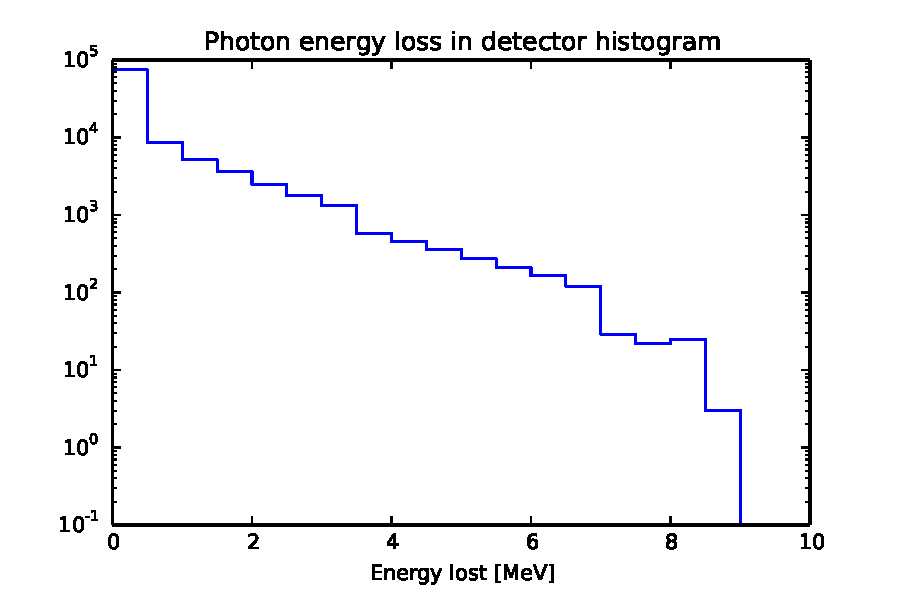
\includegraphics[width=0.7\textwidth]{fig-Eloss-hist.pdf}
    \caption{\label{fig:Eloss-hist} Energieafgifte aan detector per foton.}
  \end{center}
\end{figure}


\subsection{Analyse van de detectorresponse van fotonen per mechanisme}

\subsubsection{Analyse van de bijdrage van het foto-elektrisch effect}
In \cite*{Steijger2010-gammas} is de ondergrens van de primaire fotonon in de minimontecarlo simulatie bepaald op 100 keV. Fotonen met minder energie worden niet waargenomen, omdat PMT pulsen binnen het ruisniveau vallen.

Omdat de werkzame doorsnede voor het foto-elektrisch effect bij 100keV klein is, zijn er slechts weinig (minder dan 1\%) fotoelektrische interacties (tabel  \ref{table:mmc-mechanisme}) in de simulatie. Deze interacties leveren electronen in de scintilator plaat met lage energie (figuur \ref{fig:fe}). De bijbehorende pulshoogte is onder het ruisniveau.

\begin{figure}[h]
        \begin{subfigure}[b]{0.6\textwidth}
                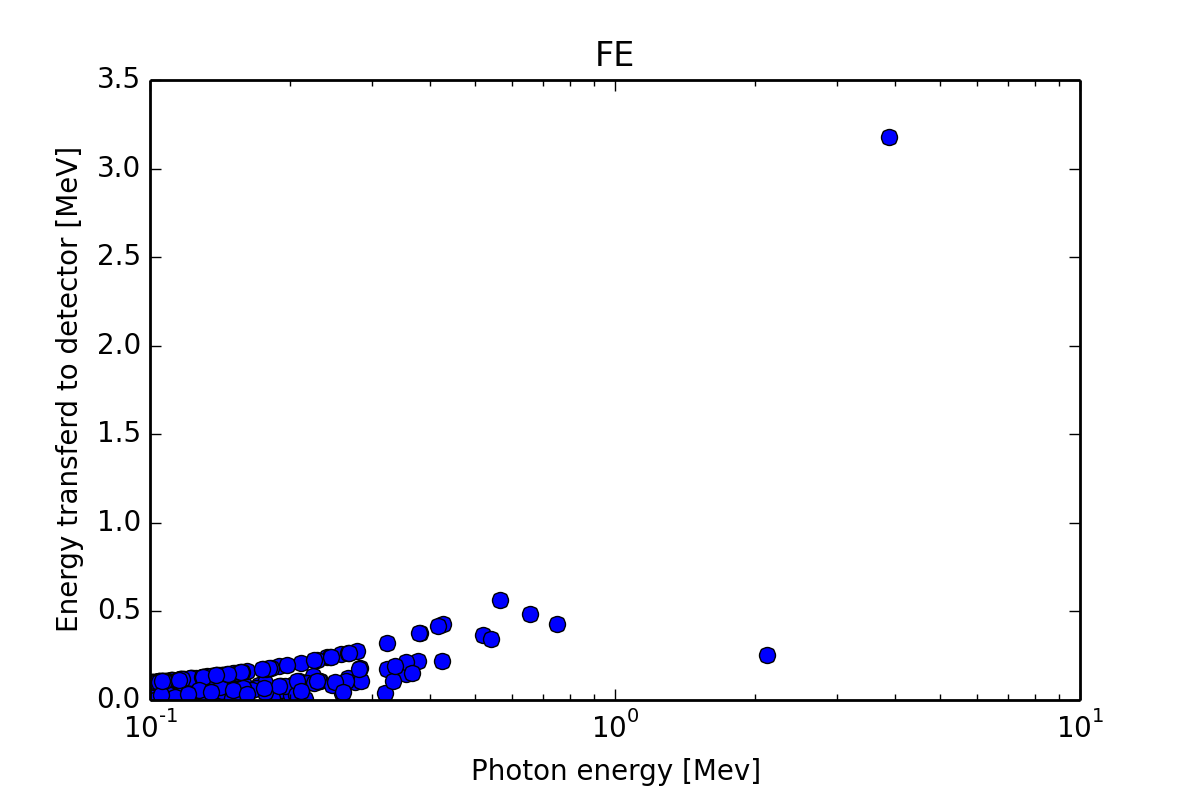
\includegraphics[width=1\textwidth]{fig-fe-scatter.png}
                \caption{Scatter plot van events}
                \label{fig:fe-scatter}
        \end{subfigure}
        \begin{subfigure}[b]{0.6\textwidth}
                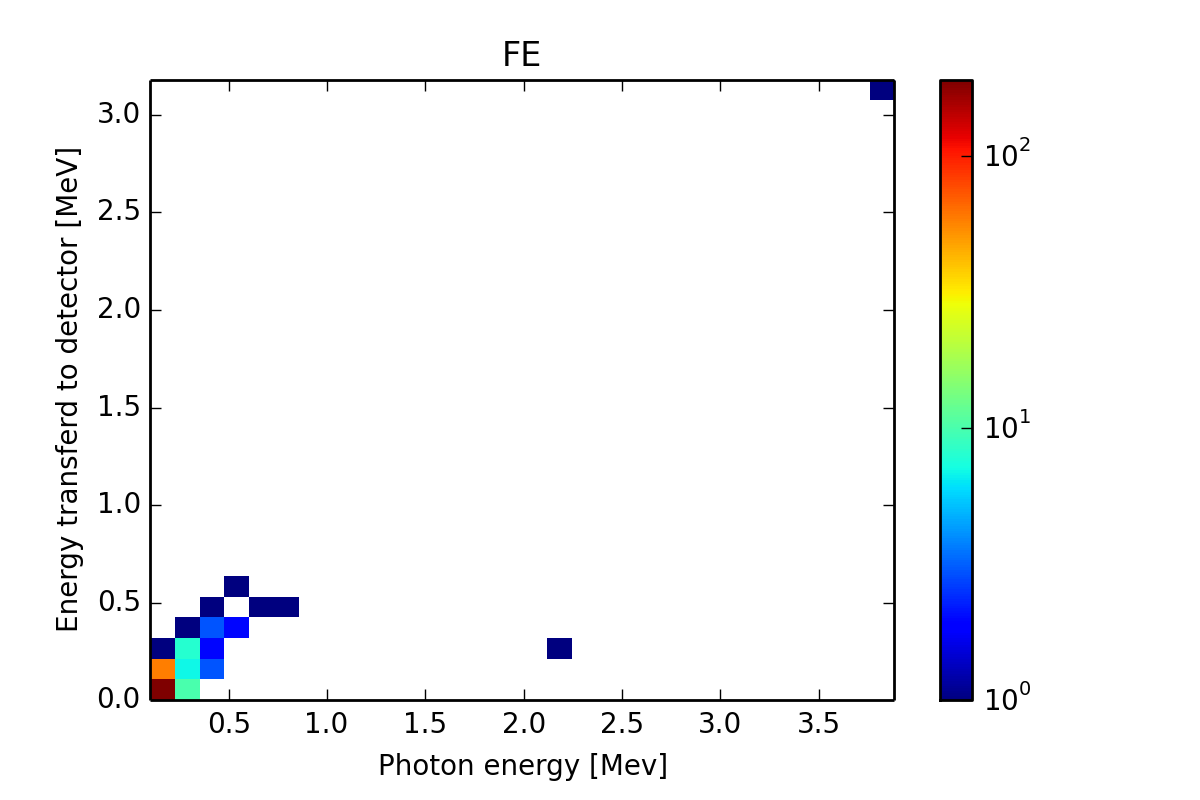
\includegraphics[width=1\textwidth]{fig-fe-hist2d.png}
                \caption{2D histogram van events}
                \label{fig:fe-hist3d}
        \end{subfigure}
        \caption{Foto-elektrisch effect: Energieoverdracht aan detector vs Gamma energie}\label{fig:fe}
\end{figure}


Conclusie: Het foto-elektrisch effect kan verwaarloosd worden.

\subsubsection{Analyse van de bijdrage van Compton verstrooiing}
Compton verstrooiing is het mechanisme dat voor 90\% van alle interacties zorgt. In figuur \ref{fig:compton-scatter}  \ref{fig:compton-hist2d} en  is de energie afgifte aan de detector weergegeven. Het overgrote deel van de energie overdracht aan de detector is tussen de 0.1 en 2 MeV. Bijbehorende pulshoogte is tussen ruis en 60mV (120 ADC counts)
\footnote{3.38 MeV = 200mV = 350 ADC counts; De hoogte van de \textit{MIP piek} is 3.38 MeV, dit komt overeen met 200mV (beide volgens \cite*{Pennink:2010} blz 24). 1mV komt overeen met 1.75 ADC stap (volgens \cite*{Pennink:2010} blz 32).}.

\begin{figure}[h]
        \begin{subfigure}[b]{0.6\textwidth}
                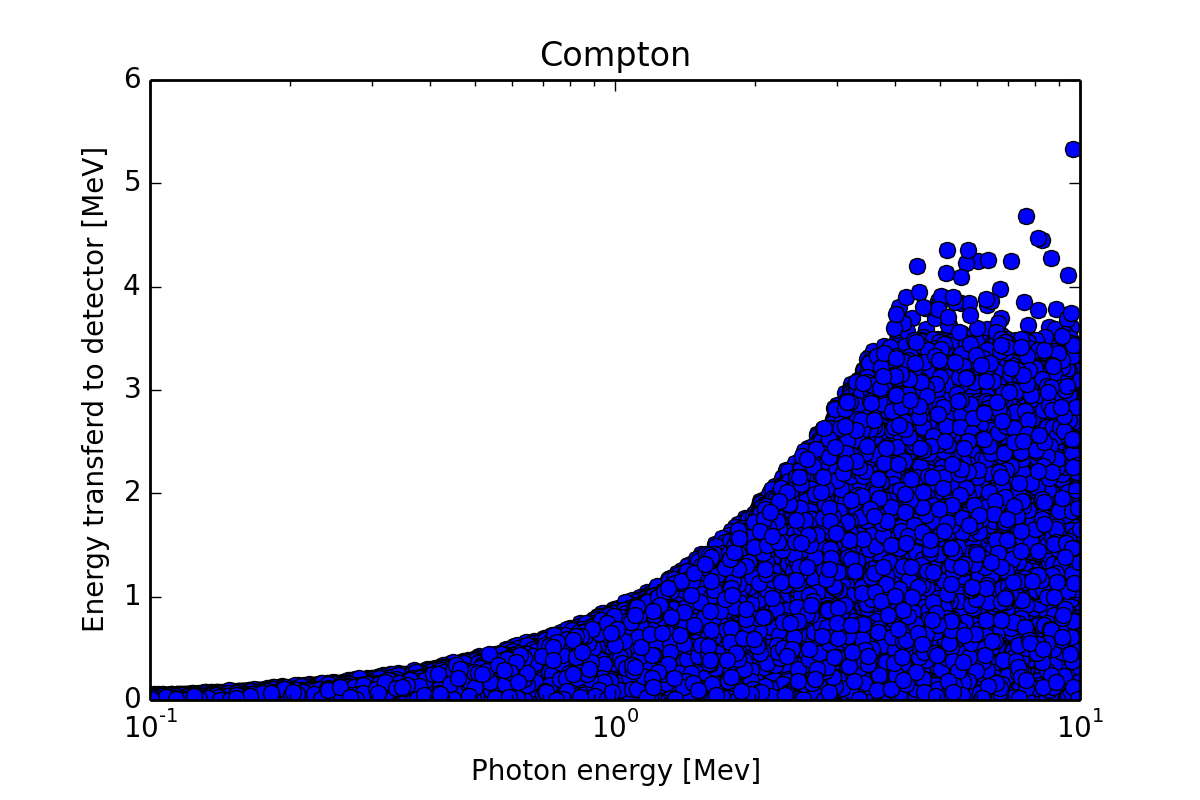
\includegraphics[width=1\textwidth]{fig-compton-scatter.png}
                \caption{Scatter plot van events}
                \label{fig:compton-scatter}
        \end{subfigure}
        \begin{subfigure}[b]{0.6\textwidth}
                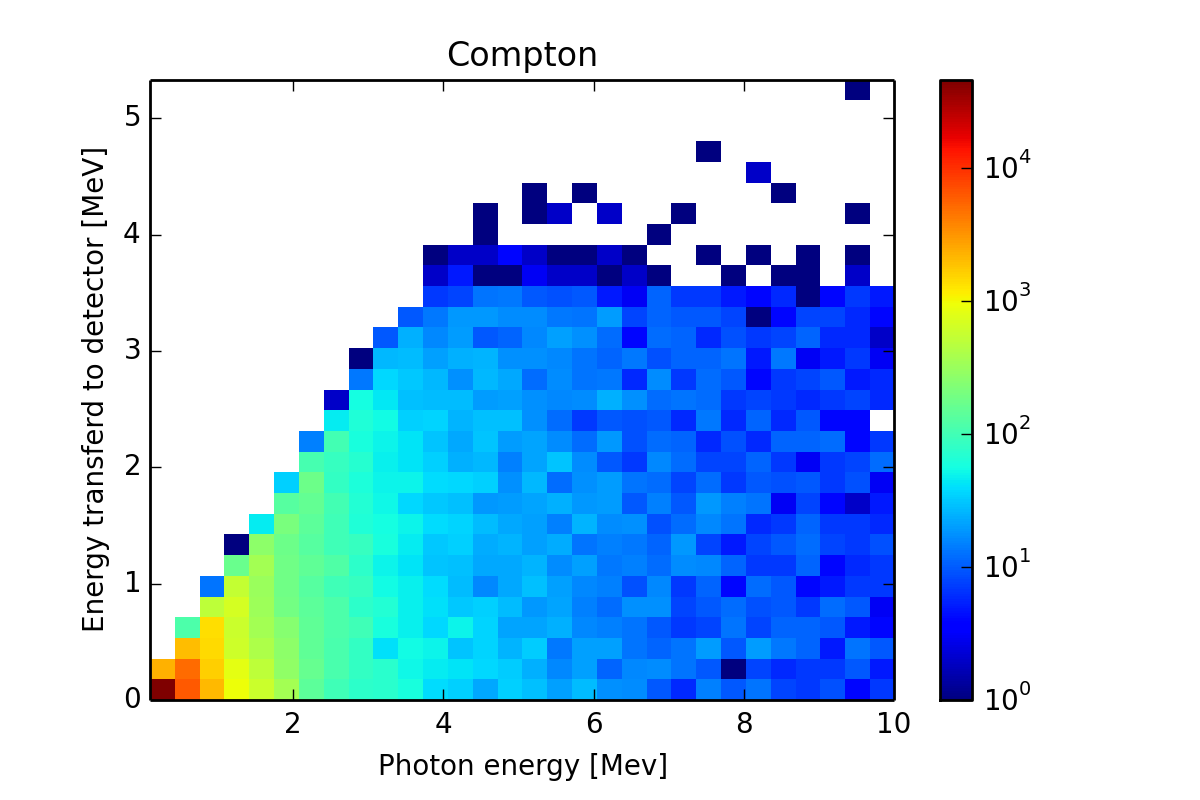
\includegraphics[width=1\textwidth]{fig-compton-hist2d.png}
                \caption{2D histogram van events}
                \label{fig:compton-hist3d}
        \end{subfigure}
        \caption{Compton verstrooiing: Energieoverdracht aan detector vs Gamma energie}\label{fig:compton}
\end{figure}


Conclusie: Compton verstrooiing zorgt voor detector response in het voor deze analyse interessante gebied.


\subsubsection{Analyse van de bijdrage van paarvorming}
Bij ongeveer 10\% van de interacties van fotonen in de detector treedt paarvorming op. De overgedragen energie is hierbij hoog. In figuren \ref{fig:pair} is af te lezen dat de energieoverdracht meestal groter is dan 2 MeV. De bijbehorende pulsehoogte is ongeveer 120mV (200 ADC counts)\footnote{3.38 MeV = 200mV = 350 ADC counts} en groter.

Daarmee zijn de pulsen ononderscheidbaar van geladen leptonen.

\begin{figure}[h]
        \begin{subfigure}[b]{0.6\textwidth}
                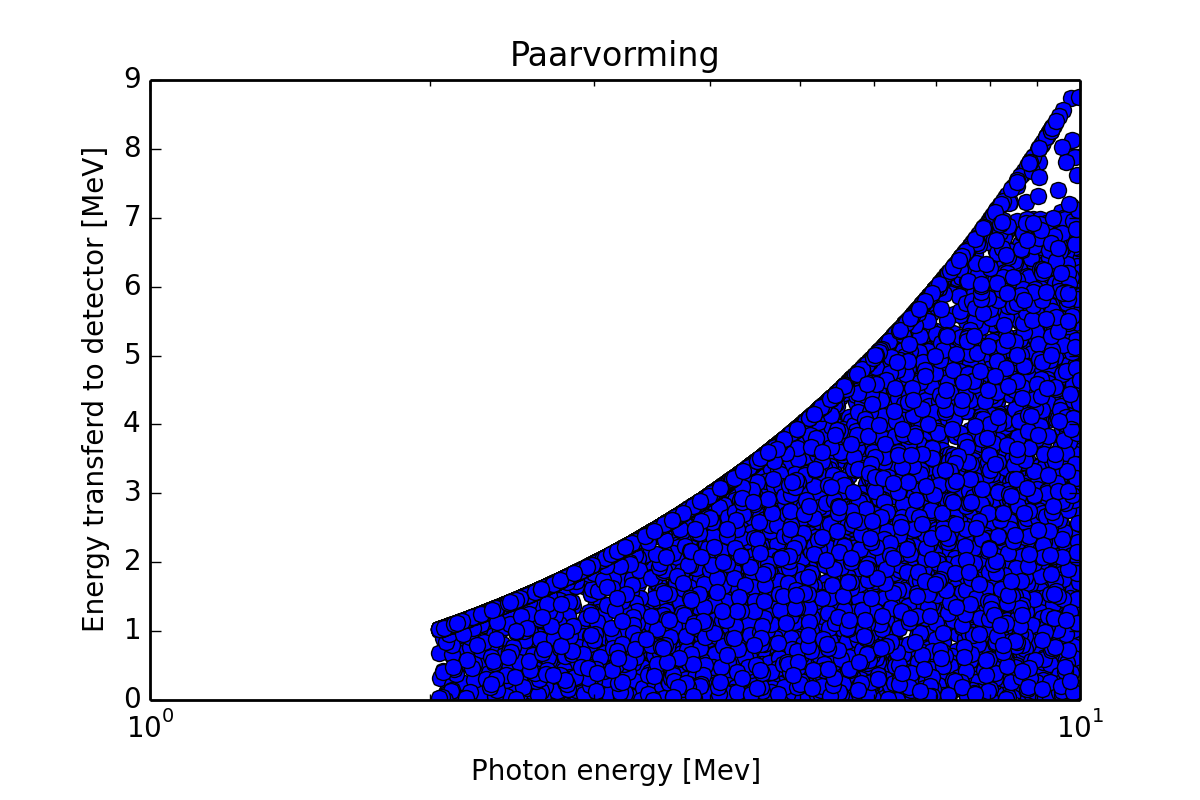
\includegraphics[width=1\textwidth]{fig-pair-scatter.png}
                \caption{Scatter plot van events}
                \label{fig:pair-scatter}
        \end{subfigure}
        \begin{subfigure}[b]{0.6\textwidth}
                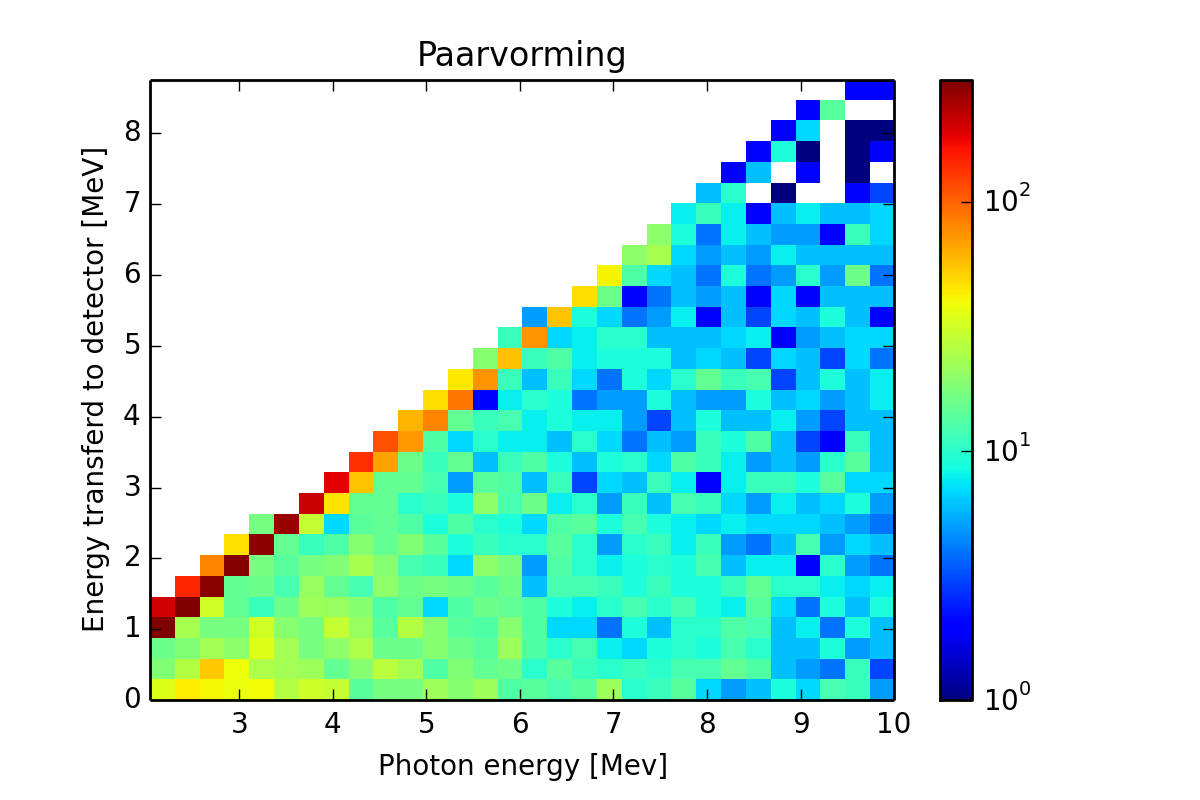
\includegraphics[width=1\textwidth]{fig-pair-hist2d.png}
                \caption{2D histogram van events}
                \label{fig:pair-hist3d}
        \end{subfigure}
        \caption{Paarvorming: Energieoverdracht aan detector vs Gamma energie}\label{fig:pair}
\end{figure}

Conclusie: Compton verstrooiing levert grote detectorrespons die onderscheidbaar is van de response door geladen leptonen. De interactiekans is echter zo klein, dat deze bijdrage t.o.v. de bijdrage van geladen leptonen verwaarloosd kan worden.








\section{Compton verstrooiing}
Uitleg compton verstrooing

Deze paragraaf vullen naar behoefte vanuit tekst hieronder
\subsection{Detectiekans}
Werkzamedoorsnede
\subsection{Afgegeven energie aan het electron}

\section{Parametrisatie}
\subsection{Detectiekans}
\subsection{Afgegeven energie}

\section{Sapphire algorithme}
Flowchart?


\bibliography{mybib}{}
\bibliographystyle{plain}


\end{document}
